%!TEX root = ../dokumentation.tex

\chapter{Continuous Delivery}

\section{Einleitung}
Dieses Kapitel beschäftigt sich mit den Grundlagen von \acl{CD}. Zum Ende dieses Kapitels werden Argumente für und gegen \acs{CD} dargestellt und ein Vergleich mit der momentanen Situation bei TwoGo durchgeführt.\\
Softwareentwicklung ist ein komplexer und mehrschichtiger Prozess (Abbildung \ref{img:Entwicklungsprozess}). In der Regel beginnt alles mit einer guten Idee, gefolgt von der Entwicklung, dem Testen der Software und schließlich dem Liefern (eng.: deliver) der Software an den Kunden.
 %\begin{wrapfigure}{r}{0.5\textwidth}
  %\vspace{-30pt}
  %\begin{center}
  %  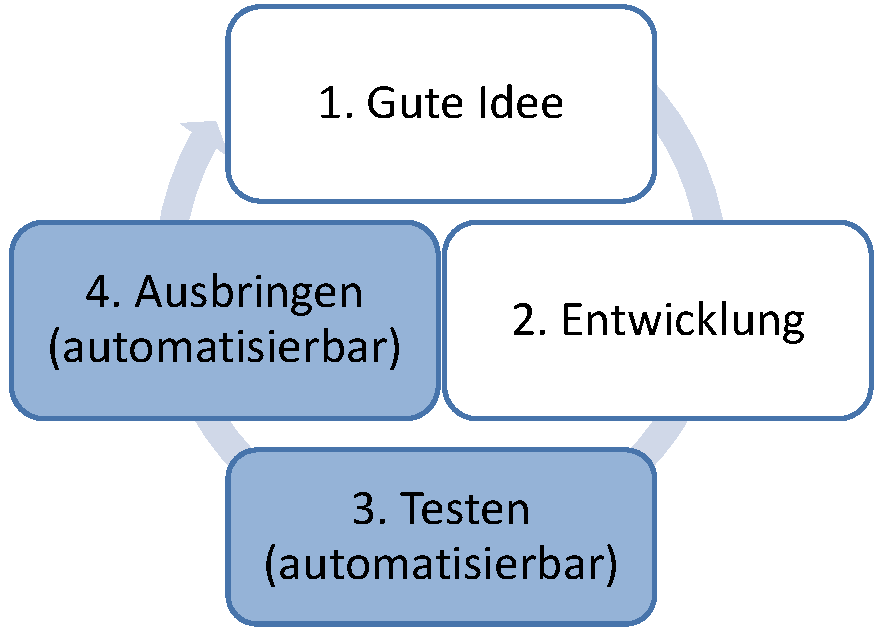
\includegraphics[width=0.55\textwidth]{Entwicklung_Prozess2.pdf}
  %\end{center}
  %\vspace{-20pt}
  %\caption{Entwicklungsprozess}
  %\vspace{-2pt}
  %\label{img:Entwicklungsprozess}
%\end{wrapfigure}
\begin{figure}[H]
    \centering
    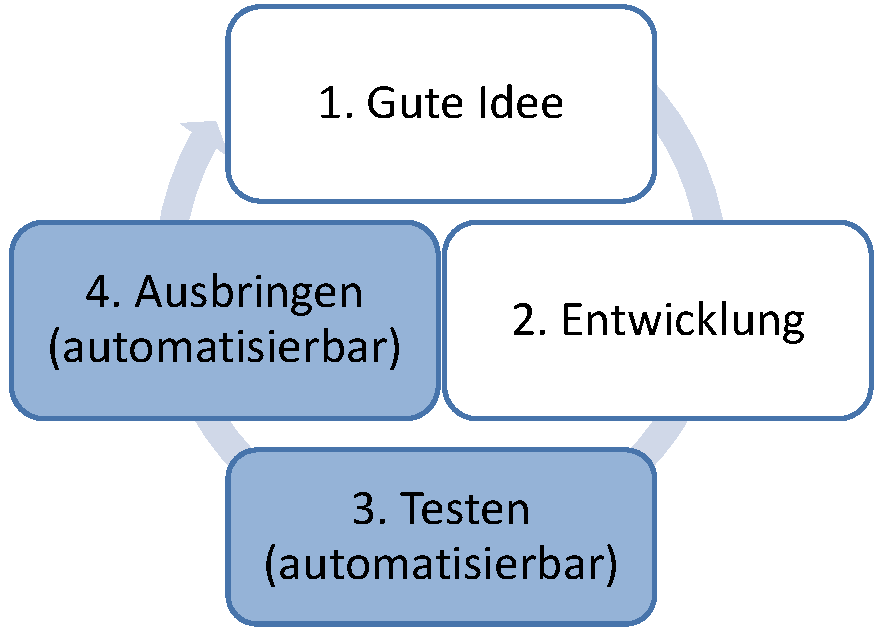
\includegraphics[width=0.6 \textwidth]{Entwicklung_Prozess2.pdf}
    \caption{Entwicklungsprozess} \cite[Seite 9 (angelehnt)]{swartout_continuous_2012}
  \label{img:Entwicklungsprozess}
\end{figure}

Für ein Softwareunternehmen ist der letzte Teil der wichtigste, denn nur wenn die Software beim Kunden produktiv eingesetzt werden kann, wird Gewinn generiert. Daraus lässt sich schließen, dass bei diesem Prozess hohe Effektivität und Geschwindigkeit  eine  entscheidende  Rolle spielen. Dieses Ziel lässt sich durch den Einsatz von \acs{CD} erreichen.\footnote{Vgl. \cite[Kapitel 1]{swartout_continuous_2012}}\\
\acs{CD} beschreibt die Optimierung dieses Prozesses und geht dabei sowohl auf technische als auch auf organisatorische Aspekte ein. Ein zentrales Merkmal von \acs{CD} ist es, Teile des Prozesses zu automatisieren und sich auf wichtige Elemente, wie das Programmieren, zu fokussieren. Der Grund für diese Überlegung ist einfach: Wieso sollte man Aufgaben, die sehr zeitaufwendig und komplex sind, manuell ausüben, wenn man diese auch automatisieren kann? \\ In vielen Teams, wie dem SAP TwoGo-Team\footnote{siehe Kapitel 2.3}, wird beispielsweise das Produkt händisch ausgebracht (eng.: deploy). Dies ist ein komplexer und aufwendiger Prozess, bei dem es leicht zu menschlichen Fehlern kommen kann. Durch die Automatisierung können diese Fehler reduziert werden und die überschüssige Arbeitskraft in wichtigeren Bereichen genutzt werden. Es wird hiermit erkennbar, wo \acs{CD} ansetzt und welche Vorteile es bietet.\footnote{Vgl. \cite[Seite 3ff]{continuous_dev}} \\
%Der Grund für diese Überlegung ist einfach, wieso sollte man Aufgaben, die sehr zeitaufwendig und komplex sind wie dem ausbringen (eng.: deploy) von Software manuell tätigen, wenn man diese auch automatisieren könnte? Durch die Automatisierung können menschliche Fehler reduziert werden und die überschüssige Arbeitskraft kann in wichtigeren Bereichen genutzt werden. Es wird hiermit erkennbar wo \ac{CD} ansetzt und welche Vorteile es bietet.\footnote{\cite{continuous_dev}} \\
Durch die vollständige Umsetzung von \acs{CD} soll es  letztendlich möglich sein, eine beliebige Version der Software mit dem Klicken eines Buttons zu einem beliebigen Zeitpunkt auszuliefern. Dabei soll auch mehrmals täglich ausgeliefert werden können, weshalb Schnelligkeit und Effektivität entscheidende Merkmale sind.\footnote{Vgl. \cite[Seite 5]{continuous_dev}} Dieser Prozess wird in der Fachliteratur   auch als \textit{deployment pipeline} beschrieben (zum Beispiel \cite{continuous_dev}).\\

\section{Deployment Pipeline}
Die Deployment Pipeline, dargestellt in Abbildung \ref{img:depl_pipe}, beschreibt einen automatisierten Prozess, welcher mit dem Freischalten einer Änderung (eng.: \textit{commit}) eines Entwicklers in das \acs{VCS} beginnt und mit dem Release der Software endet. Dazwischen erfolgen noch viele weitere Schritte, wie das Kompilieren und das Testen. Diese sind notwendig um sicherzustellen, dass der Quellcode fehlerfrei ist und produktiv eingesetzt werden kann.\footnote{Vgl. \cite[Kapitel 5]{continuous_dev}}
\begin{figure}[H]
    \centering
    \vspace{-10pt}
    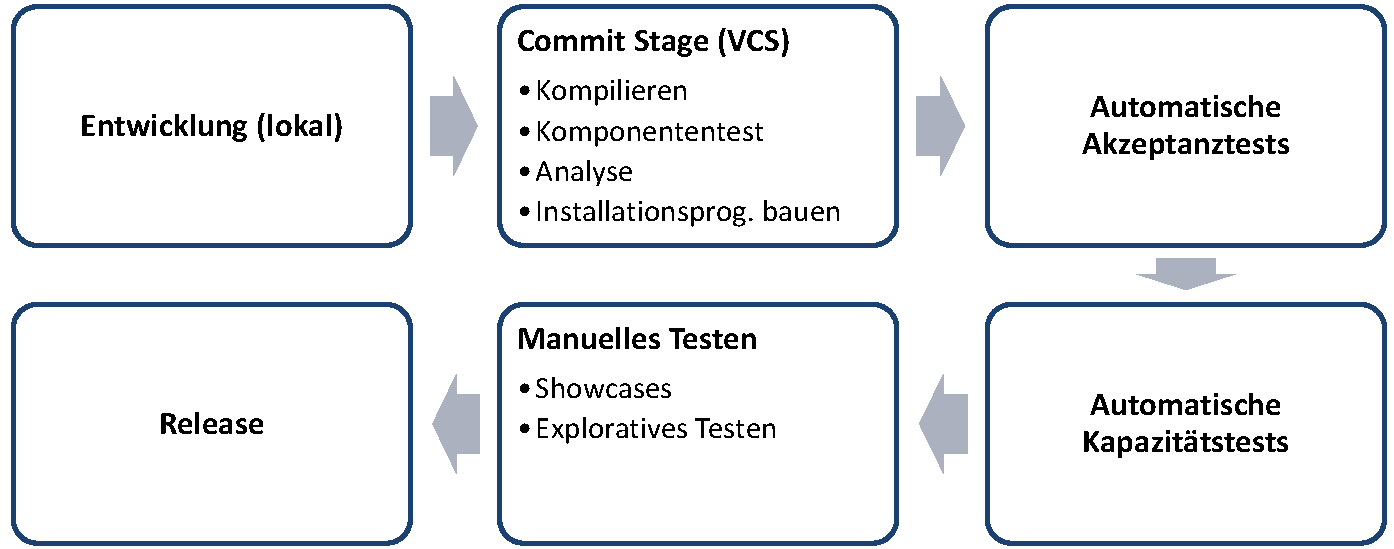
\includegraphics[width=1 \textwidth]{Deployment_Pipeline3.pdf}
    \vspace{-20pt}
    \caption{Deployment Pipeline} \cite[Seite 4 (angepasst)]{continuous_dev}
  \label{img:depl_pipe}
\end{figure}

Ein zentrales Element der Deployment Pipeline ist der Auslösezeitpunkt. Nach jedem Commit im \acs{VCS} wird diese Pipeline von neuem ausgelöst. Dadurch wird es möglich, dass jede Änderung in den Quelldateien potentiell ausgebracht  werden kann. Um einen guten Überblick zu gewährleisten, stellt jeder Durchgang der Deployment Pipeline eine neue Version der Software dar. Um die Sicherheit zu erhöhen, bleibt sowohl von den Quelldateien als auch den Binärdateien jede Version im \acs{VCS} bzw. dem zentralen Repository gespeichert. Die dadurch entstehende Historie gewährleistet, dass zu jedem Zeitpunkt eine Wiederherstellung einer älteren Version durchgeführt werden kann.\\
Für die Realisierung der Deployment Pipeline werden bestimmte Tools, wie das bereits mehrfach genannte \acs{VCS}, Skripte, Tests und organisatorische Umstrukturierungen  benötigt. Diese werden in den Unterpunkten dieses Kapitels genauer erläutert.


\subsection{Continuous Integration}
\acs{CI} (deutsch: Kontinuierliche Integration) ist ein essentieller Bestandteil der Deployment Pipeline, weil es einen großen Teil der Aufgaben übernimmt. Nach \cite{Fowler_CI} wird \acs{CI} folgendermaßen definiert (übersetzt aus dem englischen Original\footnote{Vgl. \cite[Seite 13f]{continuous_int}}): \begin{quote}
\frqq\textit{Die Kontinuierliche Integration ist eine Softwareentwicklungspraktik, bei der Teammitglieder ihre Arbeit häufig integrieren. Üblicherweise integriert jede Person im Team mindestens einmal täglich was zu mehreren Integrationen am Tag führt. Jede Integration wird durch einen vollautomatischen Build (und Test) geprüft, um Fehler so schnell wie möglich aufzudecken.}\flqq
\end{quote}
Damit diese Definition eines \acs{CI}-Systems gilt, müssen folgende Anforderungen erfüllt werden, wofür wiederum bestimmte Tools bzw. Systeme erforderlich sind. Die Anforderungen sind\footnote{Vgl. \cite{Fowler_CI} und Vgl. \cite[Seite 15f]{continuous_int}}: 
 
\begin{itemize}
\item \textit{Gemeinsame Codebasis}\\
Der gesamte Quellcode und alle weiteren Dateien, die Bestandteil der Software sind, werden an einem zentralen Ort gespeichert. Dazu wird in der Regel ein \acs{VCS} benutzt. In einem solchen System erhält jede Datei eine Versionsnummer und mit jeder Änderung wird diese erhöht. Die Besonderheit an einem \acs{VCS}  ist dabei, dass man zu jeder beliebigen Version zurückspringen kann. Dadurch kann Datenverlust verhindert werden und jeder Mitarbeiter kann immer auf den aktuellen Quellcode zurückgreifen. Bekannte \acs{VCS} Tools sind \textit{Git} oder \textit{Perforce}.

\item \textit{Vollautomatischer Build}\\
Das \acs{CI} soll aus den Quelldateien, welche es über das \acs{VCS} bekommt, vollautomatisch und bei jeder Änderung neue Binärdateien erzeugen. Dazu ruft es ein System/Tool auf, welches aus den Quelldateien Binärdateien kompiliert. Dazu können zum Beispiel  \textit{Maven} oder \textit{Ant} eingesetzt werden. Die erzeugten Binärdateien werden danach auf einem zentralen Repository gespeichert. Dieses Repository kann Bestandteil des \acs{CI} Systems sein oder befindet sich auf einem externen Server wie einem \textit{Nexus}. Für die weiteren Schritte ist es dadurch nicht mehr notwendig, Quelldateien neu zu kompilieren, da diese Zugriff auf das Repository haben.

\item \textit{Automatische Tests}\\
Laut Definition sollen mithilfe von \acs{CI} Fehler so schnell wie möglich gefunden werden. Deshalb ist es notwendig, dass das \acs{CI} System auch automatische und produktnahe Tests durchführen kann. Um möglichst viele Fehler zu finden, werden unterschiedliche Arten von Tests durchgeführt, dazu gehören Quellcodetests oder Akzeptanztests. Die Testarten werden im nächsten Kapitel näher vorgestellt. Auch bei den Tests nutzt das \acs{CI} System verschiedene Tools wie beispielsweise \textit{Selenium}.

\item \textit{Feedback}\\
Durch das kontinuierliche  Bauen und Testen bekommt der Entwickler  sehr schnell Feedback über seine Veränderungen am Quellcode. Um auf Probleme beim Bauen hinzuweisen, werden oft Ampeln oder das Abspielen von Geräuschen verwendet. Da die Veränderungen aufgrund des regelmäßigen Integrierens der Entwickler nur kleine Änderungen darstellen, kann er den Fehler schneller verstehen und beheben.
\end{itemize}

Vergleicht man diese Punkte mit den Prozessschritten der Deployment Pipeline, so erkennt man, dass bereits viele Punkte, wie das automatische Kompilieren und Testen, durch ein \acs{CI} System erfüllt werden. Mit vielen \acs{CI} Systemen, wie beispielsweise \textit{Jenkins}, ist es zudem möglich durch die korrekte Konfiguration fast alle Schritte der Deployment Pipeline abzudecken. %Wie viel das \ac{CI} System letzten Endes abdeckt, hängt davon ab welche Software eingesetzt wird. Bei manchen \ac{CI} Systemen, wie \textit{Jenkins}, ist es mit der entsprechenden Konfiguration sogar möglich die komplette Deployment Pipeline abzubilden.

\subsection{Testarten}
Ein weiterer wichtiger Bestandteil der Deployment Pipeline liegt in der automatischen oder manuellen Durchführung von Tests. Um dabei möglichst alle Fehler zu finden, ist es notwendig, mehrere Testarten einzusetzen. In der agilen Softwareentwicklung, welche bei \acs{CD} sehr nützlich  ist (siehe Kapitel 3.4.2), werden die Testarten vier unterschiedlichen Kategorien zugeordnet. Diese sind in der Matrix in Abbildung \ref{img:test_typen} dargestellt und werden nun näher erläutert.\footnote{Vgl. \cite[Kapitel 4]{continuous_dev}} %\begin{wrapfigure}{r}{0.6\textwidth}
%  \vspace{-30pt}
%  \begin{center}
%    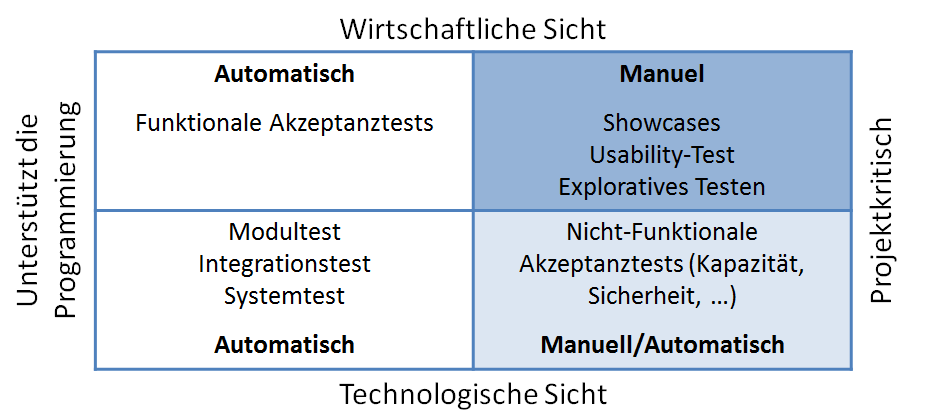
\includegraphics[width=0.6\textwidth]{Test_typen}
%  \end{center}
%  \vspace{-25pt}
%  \caption{Testarten}  \cite[Grafik 4.1 (übersetzt)]{continuous_dev}
%     \vspace{-15pt}
%  \label{img:test_typen}
%\end{wrapfigure}
\begin{figure}[H]
\vspace{-10pt}
\centering
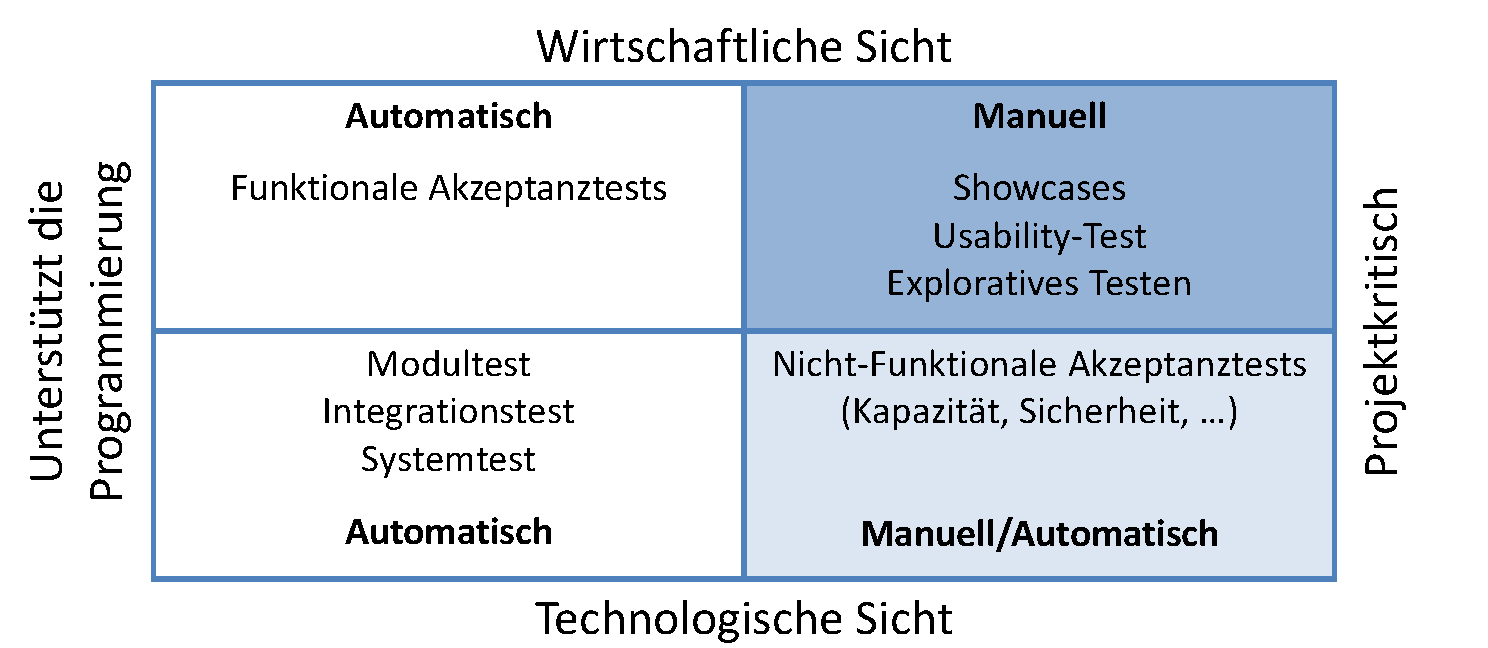
\includegraphics[width=1\linewidth]{../images/Test_typen.pdf}
\vspace{-30pt}
  \caption{Testarten}  \cite[Grafik 4.1 (übersetzt)]{continuous_dev}
  \vspace{-10pt}
\label{img:test_typen}
\end{figure}

Mit dieser Darstellung wird sichergestellt, dass möglichst alle Aspekte eines Produktes getestet werden. Generell lassen sich Tests, die Programmierer unterstützen, automatisieren und solche, die das Produkt an sich betreffen, meistens nicht automatisieren.  \\
Aus wirtschaftlicher Sicht ist es essentiell, dass alle Anwendungsfälle (eng.: Use Cases)  erfüllt werden. Als User möchte ich beispielsweise, dass sich Fenster \textit{y} öffnet, wenn ich auf den Knopf \textit{x} drücke. Dies kann man mit sogenannten automatischen Akzeptanztests testen. Verläuft dieser Test fehlerfrei, weiß der Entwickler, ob sein Code diesen Use Case erfüllt. Es gibt jedoch Aspekte eines Produktes, die man nicht automatisch testen kann, wie beispielsweise das Design oder der Bedienkomfort (eng.: Usability), da diese sehr subjektiv  und vom Endbenutzer abhängig sind. In diesem Bereich ist somit manuelles Testen unvermeidbar.\\
Bei der technischen Sicht geht es darum, dass der Code generell funktioniert und spezielle Richtlinien erfüllt. Dazu gibt es automatische Modul- und Integrationstests. Diese überprüfen einzelne bzw. mehrere Codeabschnitte, wie beispielsweise eine bzw. mehrere Java Klassen und melden so dem Entwickler eventuelle Fehler. Während die Software deployed und installiert wird, werden automatische Systemtests, zum Beispiel ein Deployment-Test, ausgeführt. Diese gewährleisten, dass das Produkt richtig installiert und konfiguriert ist und überprüfen außerdem, ob die Systemumgebung korrekt funktioniert. Auch aus technischer Sicht gibt es Aspekte, die nicht oder nur teilweise automatisch getestet werden können. Dazu gehören beispielsweise Kapazität, Verfügbarkeit und Sicherheit. \\
All diese Tests stellen sicher, dass der Entwickler schnell Feedback erhält und dass der Großteil des Quellcodes durch automatische Tests überprüft wird. Dies ist notwendig, denn jede Änderung kann nach \acs{CD} auf dem Produktivsystem deployed werden, in welchem keine Fehler auftreten sollen.


\subsection{Automatisches Deployment}
Der letzte Schritt in der Deployment Pipeline ist das automatische Deployment. Dieses wird vom Entwickler manuell über einen Knopfdruck gestartet, nachdem er eine Funktion vollständig programmiert und getestet hat. Die Aufgabe des automatischen Deployments ist es, die Binärdateien vom zentralen Repository auf die entsprechenden Server zu kopieren, die Software zu installieren und je nach Serverkonfiguration entsprechend zu konfigurieren. Zunächst einmal ist dazu das Wissen notwendig, auf welchen Systemen die Software deployed wird. Bei kleinen Projekten kann dies der Server sein, auf dem auch das \acs{CI} System läuft. Bei größeren Projekten sind dies oft mehrere Server, die auf verschiedenen Landschaften, wie beispielsweise Entwicklung, Test und Produktion, verteilt sind. Um Fehleranfälligkeit und Rechenzeit zu vermeiden ist es empfehlenswert, immer dieselben Binärdateien, unabhängig von ihrem Zielserver, zu deployen. Dies kann erreicht werden, indem diese Server in ihrer Struktur und Konfiguration gleich sind oder die Binärdateien unabhängig von diesen Merkmalen kompiliert werden. Für letzteres ist es notwendig, auf den einzelnen Servern entsprechende Konfigurationsdateien zu pflegen.\footnote{Vgl. \cite[Seite 134f]{continuous_dev} und vgl. \cite[Seite 61]{swartout_continuous_2012}}\\
Um automatisches Deployment umzusetzen, gibt es unterschiedliche Wege. Eine Möglichkeit besteht darin, selbst programmierte Skripte zu nutzen. Mit diesen ist es  beispielsweise möglich, über Netzwerkprotokolle, wie \acs{SSH}, auf die Zielserver zuzugreifen. Diese Skripte lassen sich entweder manuell aufrufen oder werden im \acs{CI} System aufgerufen. Letzteres hat den Vorteil, dass die Deployment Pipeline komplett in einem System abgedeckt werden kann. Einen weiteren Weg stellen Deployment Tools  wie \textit{ControlTier} oder \textit{BMC BladeLogic} da, welche in Verbindung mit Infrastruktur Management Tools wie \textit{Puppet} oder \textit{CfEngine}  eingesetzt werden.\footnote{Vgl. \cite[Seite 160ff]{continuous_dev}}\\
Auf welche Weise man das automatische Deployment realisiert, hängt von vielen Faktoren ab. Wichtig dabei ist, dass ein schnelles Deployment erreicht wird, um mehrmaliges deployen am Tag zu ermöglichen.
Nachdem das Deployment ausgeführt wurde, sollte noch ein Deployment-Test durchgeführt werden, um sicherzustellen, dass der gesamte Vorgang korrekt und fehlerfrei abgelaufen ist.\footnote{Vgl. \cite[Seite 163]{continuous_dev}}\\
%Dieser Test soll u.a. überprüfen, ob der Server richtig funktioniert. Dazu gehört das er erreichbar ist und auf Anfragen reagiert. Außerdem soll der Test Log-Files überprüfen um Fehler und  Warnungen beim Deployment zu entdecken. Zudem soll er noch überprüfen ob notwendige Programme, wie z.B. die Datenbank richtig funktionieren.
\subsection{Organisatorische Umstrukturierungen}
Nachdem in den vorherigen Unterpunkten primär die technischen Aspekte beleuchtet wurden, sind bei der Deployment Pipeline auch organisatorische Aspekte sehr wichtig. Denn nicht nur die technischen Anforderungen müssen erfüllt sein, sondern auch die Mitarbeiter müssen ihr Arbeitsverhalten anpassen. Grundsätzlich muss das Team in der Lage sein, sehr schnell neue Features zu entwickeln, damit die Deployment Pipeline sehr oft durchlaufen werden kann. Um dies zu erreichen, bietet sich die Agile Softwareentwicklung an, da hier der Fokus auf wichtige Elemente, wie das Programmieren, gelegt wird und nach dem \acs{KISS} (Keep it simple and stupid) Prinzip gehandelt wird.\footnote{Vgl. \cite[ Kapitel 2]{swartout_continuous_2012}}\\ In der Fachliteratur  wird dabei vor allem \textit{Kanban} als Agiler Prozess bei \acs{CD} verwendet (zum Beispiel \cite{continuous_dev} und \cite{swartout_continuous_2012}).\\
Kanban ähnelt stark dem Scrum Prozess, welcher mittlerweile bei vielen IT Unternehmen, wie auch SAP, Standard ist. Bei beiden Prozessen werden die einzelnen Funktionen einer Software in viele kleine Aufgaben aufgeteilt, damit diese schneller entwickelt werden können. Bei Scrum gibt es feste Sprint-Zyklen, welche dazu führen, dass die einzelnen Funktionen erst am Ende des Sprints fertig sind. Daraus ergibt sich, dass ein Deployment immer nur am Ende eines Sprints möglich ist. Bei Kanban gibt es diese Einschränkung nicht, das heißt eine neue Funktion kann unmittelbar nach Fertigstellung deployed werden\footnote{Vgl. \cite[Seite 50]{Kniberg2010}}. Damit ermöglicht Kanban, dass die Deployment Pipeline bei jedem abgeschlossenen neuen Teil von neuem angestoßen werden kann.

\section{Bewertung von Continuous Delivery}
Kapitel 3.2 hat verdeutlicht, dass viele technische Eingriffe und organisatorische Umstrukturierungen notwendig sind, um ein erfolgreiches \acs{CD} umzusetzen. Dementsprechend hat \acs{CD} neben vielen Vorteilen auch einige Nachteile, die im Folgenden dargestellt werden. \\
Zu den Nachteilen gehört primär der hohe Aufwand \acs{CD} umzusetzen. Zum einen müssen viele Programme bzw. Systeme, wie das \acs{CI} System oder das \acs{VCS}  Tool, installiert und eingerichtet werden. Bis diese alle Spezifikationen erfüllen und fehlerfrei laufen, können mehrere Wochen vergehen. Zudem sind für diese Programme/Systeme eventuell auch  Softwarelizenzen oder Hardware, wie zum Beispiel Server, erforderlich. Es entsteht somit neben einem hohen zeitlichen Aufwand auch ein finanzieller Aufwand. Auch die manuellen und automatischen Tests müssen erstellt, beziehungsweise modifiziert werden und die Skripte für das automatische Deployment müssen geschrieben werden, damit alle Schritte der Deployment Pipeline abgedeckt sind. All dies zeigt, dass viele technische Veränderungen notwendig sind. Dabei muss gewährleistet sein, dass alle Elemente fehlerfrei laufen, damit die eigentliche Entwicklung der Software reibungslos ablaufen kann. Auch aus Team-Sicht entstehen Nachteile. Das Team muss unter Umständen auf einen völlig neuen Entwicklungsprozess umsteigen. Solche radikalen Veränderungen führen am Anfang dazu, dass vieles langsamer und ineffektiver abläuft. Im schlimmsten Fall verzögern einige Teammitglieder diese Veränderung, weil sie gegen eine Umsetzung von \acs{CD} sind oder bei gewohnten Vorgehensweisen bleiben möchten. \\
Es gibt jedoch auch viele positive Aspekte. Nachdem \acs{CD} vollständig umgesetzt ist, können neue Funktionen innerhalb von wenigen Minuten deployed werden. Dies führt dazu, dass der Anwender sehr schnell von diesen profitieren kann. Damit verbunden ist auch, dass finanzielle Forderungen früher beglichen werden. Zugleich kann es auch ein Vorteil gegenüber der Konkurrenz sein, da man Kundenwünsche in kurzer Zeit umsetzen kann. Auch während der Entwicklung entstehen Vorteile, weil diese gegenüber klassischen Entwicklungsmodellen durch das Wegfallen von Wartezeiten viel effektiver ist. Neue Entwicklungen können damit unmittelbar nach Fertigstellung deployed werden. Zudem profitieren die Entwickler von \acs{CD}, da sie sehr schnell Feedback über ihre Veränderungen im Code bekommen. Es ist für sie dann leichter, den Fehler nachzuvollziehen und zu beheben, da die Veränderungen immer recht gering sind. Durch das Trennen der Binärdaten von den Konfigurationsdaten  wird zudem sichergestellt, dass der Code auf jedem weiteren System läuft. Sollte es bei diesen schnellen Deployments trotz diverser Tests zu Problemen kommen oder ein Kunde wünscht sich eine ältere Version, ist es durch das zentrale Repository möglich, in kürzester Zeit eine ältere Version zu deployen. \\
Insgesamt betrachtet überwiegen für mich die Vorteile, da die Nachteile keine Rolle mehr spielen, sobald \acs{CD} komplett umgesetzt ist. Natürlich muss man, gerade während der Umsetzung, auch die Nachteile beachten und muss mit einer gewissen Einführungszeit rechnen, bis alles korrekt funktioniert. Nach dieser Phase hat man aber die Möglichkeit, neue Funktionen sehr schnell zu deployen und überflüssige Wartezeiten werden vermieden.


\section{Vergleich}
In den Kapiteln 3.1 bis 3.3 wurden die Merkmale von \acs{CD} ausführlich dargestellt, erläutert und bewertet. Kapitel 2.2 stellte die verwendeten Systeme von TwoGo vor und Kapitel 2.3 beleuchtete den aktuelle Deployment Prozess von TwoGo. Dieses Kapitel vergleicht diese Themen nun, um zu ermitteln, welche Schritte bei TwoGo noch notwendig sind, um \acs{CD} vollständig umzusetzen. \\
Wie man Kapitel 2.2 entnehmen kann, nutzt TwoGo bereits viele Programme, die für \acs{CD} notwendig sind. Das Team nutzt ein zentrales \acs{VCS} System, ein Tool zum Kompilieren der Quelldateien und ein zentrales Repository, auf welchem die Binärdaten gespeichert werden. Um diese Tools zu verbinden, wird ein \acs{CI} System eingesetzt. In diesem sind ebenfalls automatische Akzeptanz-, Modul- und Integrationstests vorhanden, welche bei jedem Build-Vorgang aufgerufen werden. Das Deployment auf die Entwicklungs-, Test- bzw. Produktivlandschaft wird mithilfe eines Skripts bewerkstelligt. Dabei ist die Konfiguration der Test- und Produktivlandschaft identisch. Für das Feedback an die Entwickler werden bei Fehlschlag oder Erfolg Sounddateien abgespielt.\\
Anhand dieser Punkte zeigt sich, dass alle notwendigen Systeme für ein funktionierendes \acs{CD} vorhanden sind und auch schon vieles für ein erfolgreiches \acs{CD} getan wurde.\\
Andererseits fehlen immer noch einige Elemente und es gibt unternehmensbedingte Hindernisse. Zu letzteren gehören alle in Kapitel 2.3 beschriebenen internen Regelungen, die den Deploymentprozess verzögern und somit \acs{CD} momentan grundsätzlich verhindern. Zudem ist auch die organisatorische Struktur innerhalb des Teams nicht gänzlich auf \acs{CD} ausgerichtet. Um dies zu ändern, müsste der Softwareentwicklungsprozess von Scrum auf Kanban geändert werden. Da beides sehr ähnlich ist, sollte eine Umstellung kein größeres Problem darstellen. Mit dieser Veränderung dürfen die manuellen Tests nicht mehr, wie bisher, vom gesamten Team ausgeführt werden, sondern sollten von den einzelnen Entwicklern nach Fertigstellung ihrer Funktion selbst durchgeführt werden.\\
 Auf der technischen Seite sind ebenfalls Probleme vorhanden. So dürfen die Binärdateien nicht mehrmals gebaut werden. Dieses Problem kann gelöst werden, indem die Konfigurationsdateien, welche Bestandteil der Binärdateien sind, auf die Server ausgelagert werden. Damit die verwendeten open-source Bibliotheken immer in der richtigen Version verfügbar sind, müssen diese korrekt verwaltet werden, wie beispielsweise über den zentralen SAP Nexus. \\
Das vollautomatische Deployment auf den Entwicklungsserver ist bereits möglich, aber auf die Server innerhalb der \acs{DMZ} ist dies aufgrund der Sicherheitsrichtlinien nicht möglich. Der Zugriff müsste entweder automatisiert ablaufen oder die Sicherheitsrichtlinien müssten reduziert werden, um den Zugriff zu vereinfachen. Zudem fehlt dem Deploymentskript momentan ein zentrales Element: der Deployment-Test. Durch dessen Fehlen ist es nur durch manuelles Überprüfen möglich festzustellen, ob das Deployment erfolgreich war.